
\documentclass[12pt,a4paper]{report}

%===========================================================
% PACKAGES
%===========================================================

\usepackage{graphicx}
\usepackage{float}
\usepackage{amsmath}
\usepackage{amssymb}
\usepackage{booktabs}
\usepackage{multirow}
\usepackage{array}
\usepackage{longtable}
\usepackage{tabularx}
\usepackage{caption}
\usepackage{subcaption}
\usepackage{enumitem}
\usepackage{hyperref}
\usepackage{geometry}
\usepackage{setspace}
\usepackage{fancyhdr}
\usepackage{tikz}
\usepackage{xcolor}
\usepackage{comment}

\usetikzlibrary{
	positioning,
	arrows.meta,
	calc,
	shapes.geometric,
	shapes.misc,
	fit,
	backgrounds,
	decorations.pathmorphing
}

\geometry{
	left=1in,
	right=1in,
	top=1in,
	bottom=1in
}

\setlength{\headheight}{15pt}
\onehalfspacing


\begin{document}
	
\begin{figure}[H]
	\centering
	\resizebox{\linewidth}{!}{%
		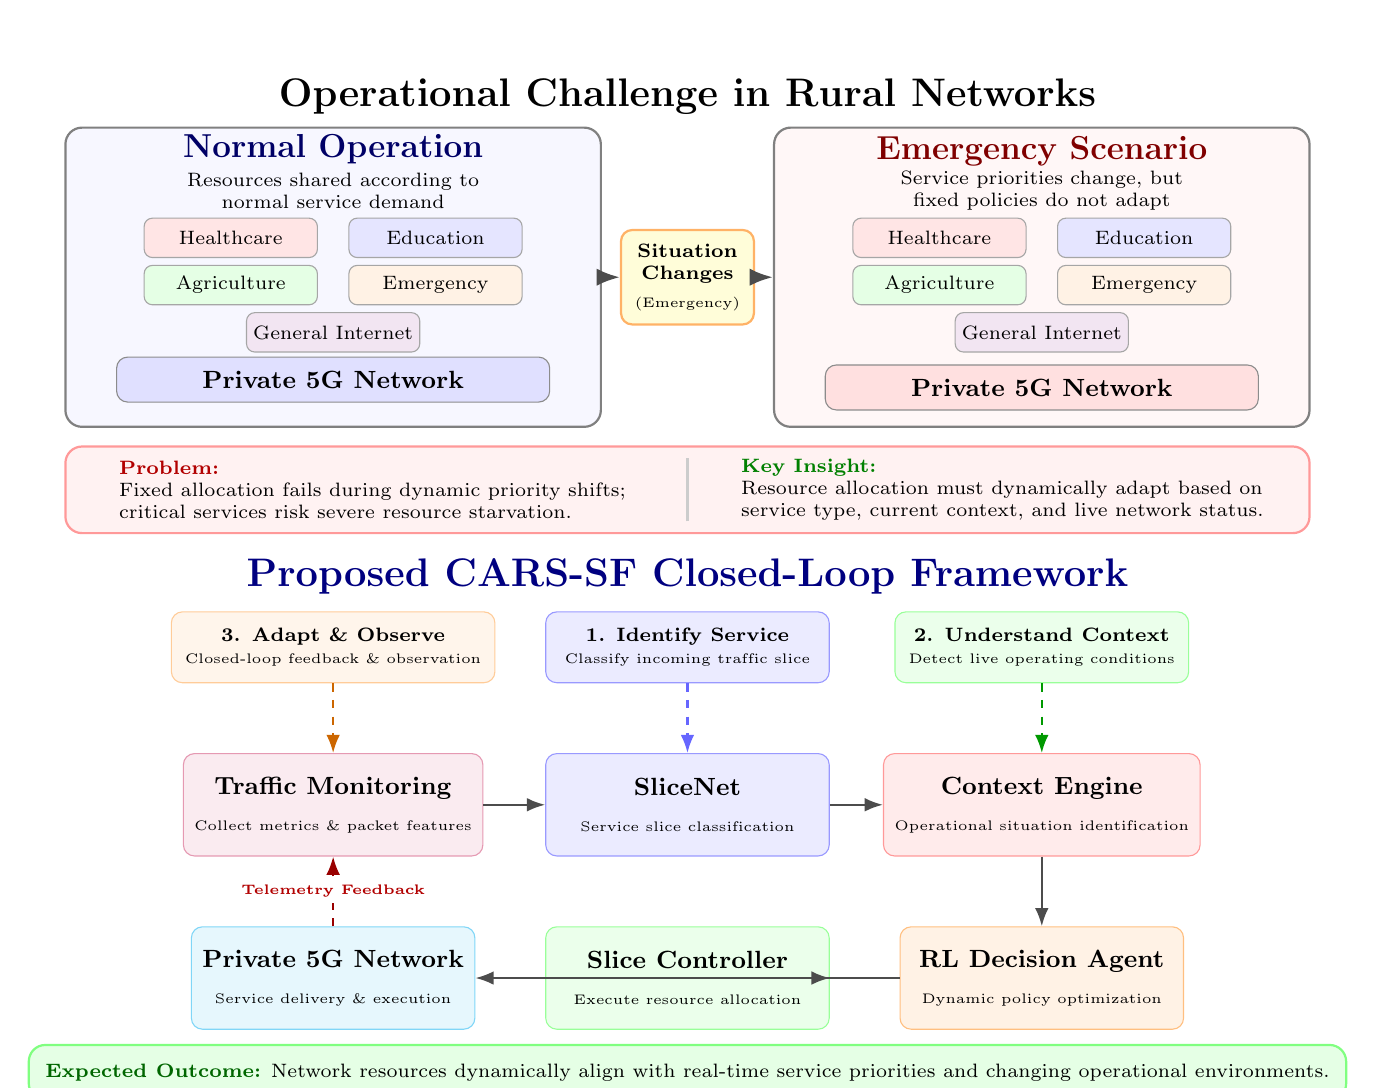
\begin{tikzpicture}[
			x=1cm,
			y=1cm,
			font=\small,
			>=Latex,
			panel/.style={
				rounded corners=6pt,
				draw=black!50,
				line width=0.8pt,
				inner sep=6pt
			},
			box/.style={
				rectangle,
				rounded corners=4pt,
				draw=black!45,
				align=center,
				inner sep=5pt
			},
			service/.style={
				rectangle,
				rounded corners=3pt,
				draw=black!35,
				minimum width=2.2cm,
				minimum height=0.5cm,
				align=center,
				font=\scriptsize,
				inner sep=2pt
			},
			module/.style={
				rectangle,
				rounded corners=4pt,
				draw=black!50,
				minimum width=2.4cm,
				minimum height=1.5cm,
				align=center,
				inner sep=4pt
			},
			arrow/.style={
				->,
				thick,
				black!70
			},
			dashedarrow/.style={
				->,
				thick,
				dashed,
				black!60
			}
			]
			
			% ========================================================
			% MAIN TITLE
			% ========================================================
			\node[font=\bfseries\Large, align=center] at (8, 0) {Operational Challenge in Rural Networks};
			
			% ========================================================
			% TOP SECTION: NORMAL vs EMERGENCY
			% ========================================================
			
			% Normal Operation Panel
			\node[panel, fill=blue!3, minimum width=6.8cm, minimum height=3.8cm] (normalpanel) at (3.5, -2.3) {};
			\node[font=\bfseries\large, color=blue!40!black] at (3.5, -0.68) {Normal Operation};
			\node[align=center, font=\scriptsize] at (3.5, -1.2) {Resources shared according to\\normal service demand};
			
			\node[service, fill=red!10] at (2.2, -1.8) {Healthcare};
			\node[service, fill=blue!10] at (4.8, -1.8) {Education};
			\node[service, fill=green!10] at (2.2, -2.4) {Agriculture};
			\node[service, fill=orange!10] at (4.8, -2.4) {Emergency};
			\node[service, fill=violet!10] at (3.5, -3.0) {General Internet};
			\node[box, fill=blue!12, minimum width=5.5cm] at (3.5, -3.6) {\textbf{Private 5G Network}};
			
			% Situation Transition
			\node[box, fill=yellow!15, draw=orange!60, line width=0.8pt, font=\bfseries\scriptsize, align=center] (change) at (8, -2.3) {Situation\\Changes\\[2pt]\normalfont\tiny (Emergency)};
			\draw[arrow, line width=1.2pt] (normalpanel.east) -- (change.west);
			
			% Emergency Scenario Panel
			\node[panel, fill=red!3, minimum width=6.8cm, minimum height=3.8cm] (emergpanel) at (12.5, -2.3) {};
			\node[font=\bfseries\large, color=red!50!black] at (12.5, -0.7) {Emergency Scenario};
			\node[align=center, font=\scriptsize] at (12.5, -1.2) {Service priorities change, but\\fixed policies do not adapt};
			
			\node[service, fill=red!10] at (11.2, -1.8) {Healthcare};
			\node[service, fill=blue!10] at (13.8, -1.8) {Education};
			\node[service, fill=green!10] at (11.2, -2.4) {Agriculture};
			\node[service, fill=orange!10] at (13.8, -2.4) {Emergency};
			\node[service, fill=violet!10] at (12.5, -3.0) {General Internet};
			\node[box, fill=red!12, minimum width=5.5cm] at (12.5, -3.7) {\textbf{Private 5G Network}};
			\draw[arrow, line width=1.2pt] (change.east) -- (emergpanel.west);
			
			% ========================================================
			% MIDDLE SECTION: PROBLEM & KEY INSIGHT
			% ========================================================
			\node[panel, fill=red!5, draw=red!40, minimum width=15.8cm, minimum height=1.1cm] (problem) at (8, -5.0) {};
			
			\node[align=left, font=\scriptsize] at (4.0, -5.0) {
				\textbf{\color{red!70!black}Problem:}\\
				Fixed allocation fails during dynamic priority shifts;\\
				critical services risk severe resource starvation.
			};
			
			\draw[line width=0.8pt, black!20] (8, -5.4) -- (8, -4.6);
			
			\node[align=left, font=\scriptsize] at (12.0, -5.0) {
				\textbf{\color{green!50!black}Key Insight:}\\
				Resource allocation must dynamically adapt based on\\
				service type, current context, and live network status.
			};
			
		% ========================================================
		% BOTTOM SECTION: PROPOSED SOLUTION (3x3 GRID ORIENTATION)
		% ========================================================
		\node[font=\bfseries\Large, color=blue!50!black] at (8.0, -6.1) {Proposed CARS-SF Closed-Loop Framework};
		
		% --------------------------------------------------------
		% ROW 1: System Requirements (Inputs)
		% --------------------------------------------------------
		\node[box, fill=orange!8, draw=orange!40, minimum width=3.6cm, minimum height=0.9cm, align=center, font=\scriptsize] (req3) at (3.5, -7.0) {
			\textbf{3. Adapt \& Observe}\\
			\tiny Closed-loop feedback \& observation
		};
		
		\node[box, fill=blue!8, draw=blue!40, minimum width=3.6cm, minimum height=0.9cm, align=center, font=\scriptsize] (req1) at (8.0, -7.0) {
			\textbf{1. Identify Service}\\
			\tiny Classify incoming traffic slice
		};
		
		\node[box, fill=green!8, draw=green!40, minimum width=3.6cm, minimum height=0.9cm, align=center, font=\scriptsize] (req2) at (12.5, -7.0) {
			\textbf{2. Understand Context}\\
			\tiny Detect live operating conditions
		};
		
		% --------------------------------------------------------
		% ROW 2: Perception & Classification (Left -> Right)
		% --------------------------------------------------------
		\node[module, fill=purple!8, draw=purple!40, minimum width=3.6cm, minimum height=1.3cm] (monitor) at (3.5, -9.0) {
			\textbf{Traffic Monitoring}\\[2pt]
			\tiny Collect metrics \& packet features
		};
		
		\node[module, fill=blue!8, draw=blue!40, minimum width=3.6cm, minimum height=1.3cm] (slicenet) at (8.0, -9.0) {
			\textbf{SliceNet}\\[2pt]
			\tiny Service slice classification
		};
		
		\node[module, fill=red!8, draw=red!40, minimum width=3.6cm, minimum height=1.3cm] (context) at (12.5, -9.0) {
			\textbf{Context Engine}\\[2pt]
			\tiny Operational situation identification
		};
		
		% --------------------------------------------------------
		% ROW 3: Decision, Control & Execution (Right -> Left)
		% --------------------------------------------------------
		\node[module, fill=cyan!10, draw=cyan!50, minimum width=3.6cm, minimum height=1.3cm] (network) at (3.5, -11.2) {
			\textbf{Private 5G Network}\\[2pt]
			\tiny Service delivery \& execution
		};
		
		\node[module, fill=green!8, draw=green!40, minimum width=3.6cm, minimum height=1.3cm] (controller) at (8.0, -11.2) {
			\textbf{Slice Controller}\\[2pt]
			\tiny Execute resource allocation
		};
		
		\node[module, fill=orange!10, draw=orange!50, minimum width=3.6cm, minimum height=1.3cm] (rl) at (12.5, -11.2) {
			\textbf{RL Decision Agent}\\[2pt]
			\tiny Dynamic policy optimization
		};
		
		% --------------------------------------------------------
		% Connections & Serpentine Closed-Loop Flow
		% --------------------------------------------------------
		% Vertical Requirement Injections (Row 1 -> Row 2)
		\draw[dashedarrow, color=orange!80!black] (req3.south) -- (monitor.north);
		\draw[dashedarrow, color=blue!60] (req1.south) -- (slicenet.north);
		\draw[dashedarrow, color=green!60!black] (req2.south) -- (context.north);
		
		% Row 2 Forward Flow (Left to Right)
		\draw[arrow] (monitor.east) -- (slicenet.west);
		\draw[arrow] (slicenet.east) -- (context.west);
		
		% Downward Transition (Col 3: Row 2 -> Row 3)
		\draw[arrow] (context.south) -- (rl.north);
		
		% Row 3 Action Flow (Right to Left)
		\draw[arrow] (rl.west) -- (controller.west |- rl.west) -- (controller.east);
		\draw[arrow] (controller.west) -- (network.east);
		
		% Upward Closed-Loop Feedback Path (Col 1: Row 3 -> Row 2)
		\draw[->, thick, dashed, red!60!black] (network.north) -- (monitor.south) 
		node[midway, fill=white, inner sep=2pt, font=\tiny\bfseries, text=red!70!black] {Telemetry Feedback};
			% Outcome Summary Box
			\node[panel, fill=green!10, draw=green!50, minimum width=15.8cm, minimum height=0.7cm, font=\scriptsize] at (8, -12.4) {
				\textbf{\color{green!40!black}Expected Outcome:} Network resources dynamically align with real-time service priorities and changing operational environments.
			};
			
		\end{tikzpicture}%
	}
	\caption{Operational challenge in rural networks and the proposed CARS-SF closed-loop framework for service-aware and context-aware resource management.}
	\label{fig:cars_sf_framework}
\end{figure}

\end{document}